\documentclass[11pt]{article}
% ---------- Packages ----------
\usepackage[letterpaper, margin=1in]{geometry}
\usepackage[utf8]{inputenc}
\usepackage[T1]{fontenc}
\usepackage{titlesec}
\usepackage{titling}
\usepackage{enumitem}
\usepackage{longtable}
\usepackage{array}
\usepackage{xcolor}
\usepackage{colortbl}
\usepackage{graphicx}
\usepackage{caption}
\usepackage{hyperref}
\usepackage{xurl}
\usepackage{tocloft}
\usepackage{fancyhdr}
\usepackage{parskip}
\usepackage{tcolorbox}
\tcbuselibrary{skins,breakable}
% ---------- Palette (matches the deck / docx template) ----------
\definecolor{navy}{HTML}{1E2761}
\definecolor{amber}{HTML}{D98C1F}
\definecolor{muted}{HTML}{6B7590}
\definecolor{lighttint}{HTML}{EFF4FE}
\definecolor{writeitred}{HTML}{B23A48}
% ---------- Headings ----------
\titleformat{\section}{\Large\bfseries\color{navy}}{\thesection.}{0.5em}{}
\titleformat{\subsection}{\large\bfseries\color{navy}}{\thesubsection}{0.5em}{}
\setlength{\parskip}{0.6em}
% ---------- Header/footer ----------
\pagestyle{fancy}
\fancyhf{}
\renewcommand{\headrulewidth}{0pt}
\fancyfoot[C]{\small\color{muted}\thepage}
% ---------- Hyperlinks ----------
\hypersetup{
  colorlinks=true,
  linkcolor=navy,
  urlcolor=navy,
  citecolor=navy,
  pdftitle={A Taxonomy of Failure Modes in Vision-Language Desktop Agents},
  pdfauthor={Zeyd Belayouni}
}
\newtcolorbox{writeit}{
  breakable, enhanced,
  colback=writeitred!7, colframe=writeitred,
  boxrule=0pt, leftrule=2.5pt,
  fontupper=\small\color{writeitred!85!black},
  arc=0pt, outer arc=0pt,
  left=8pt, right=8pt, top=6pt, bottom=6pt,
}
\newtcolorbox{datanote}{
  breakable, enhanced,
  colback=lighttint, colframe=navy!40,
  boxrule=0pt, leftrule=2.5pt,
  fontupper=\small\color{navy!80!black},
  arc=0pt, outer arc=0pt,
  left=8pt, right=8pt, top=6pt, bottom=6pt,
}
\newcolumntype{P}[1]{>{\raggedright\arraybackslash}p{#1}}
\title{
  {\Huge\bfseries\color{navy} A Taxonomy of Failure Modes in\\ Vision-Language Desktop Agents}\\[0.4cm]
  {\Large\itshape\color{muted} A Two-Month Case Study}
}
\author{Zeyd Belayouni \\ \small\color{muted} Supervised by Deborah Yuen}
\date{August 2026}
\begin{document}
\maketitle
\newpage
\tableofcontents
\newpage
\section*{Abstract}
\addcontentsline{toc}{section}{Abstract}
We built and ran a vision-language desktop agent over two months, logging every real task it attempted. Rather than treating failed runs as noise to retry, we read each one in full and traced it back to a specific, fixable cause, which surfaced eight distinct, recurring failure modes. The most consequential of these turned out to be a single weakness in our safety gate that failed in two opposite directions: a keyword-dependent confirmation check let one genuinely risky action through unconfirmed, while later flooding an unrelated, harmless sequence of actions with repeated confirmation prompts until the operator stopped trusting them and declined the one that may have mattered. We built and measured a three-layer fix for this asymmetry, verified against the exact reasoning text of the run that exposed it. This pattern of oversight fatigue is treated more formally, and independently, in concurrent 2026 work (Turan, ``Oversight Has a Capacity''); we do not claim to be first to notice it, only to document one real, grounded, shipped instance of it end to end.
\section{Introduction}
\label{sec:intro}
A vision-language desktop agent is a real-time AI agent that receives a task, reads the current contents of the screen, and works through the task step by step until it is done or gives up. Most public discussion of these systems comes from companies publishing polished, runnable demos of an agent succeeding -- not from any account of what went wrong along the way. Every agent produces its own idiosyncratic failures, which are hard to package into a compelling story, while a working demo is immediately legible to anyone watching; and there is little incentive to publish a failure once you've already shown the success. This paper takes the opposite approach.
We started by testing our agent against what it could actually do, rather than assuming it worked, and treated every failure as a piece of a larger puzzle to be root-caused and fixed in the code. This produced eight distinct, reproducible failure modes over two months of real use, each traced to a specific cause and verified with an automated regression test.
Two real runs illustrate why this is worth reading rather than filed away as routine bug-fixing. In one, asked to switch from a code editor to a browser, the agent decided the fastest path was to close the current application outright: it pressed Alt+F4 with zero confirmation, because its own explanation -- close this application to proceed -- never touched a word our safety check was listening for. In another, composing an email, the opposite problem appeared: the confirmation prompt kept firing on ordinary, harmless actions -- typing, clicking -- not because they were risky, but because the model's own reasoning kept referencing an earlier failed attempt. After enough of these, the operator stopped trusting the prompts and declined the one that may have actually mattered. The same keyword-dependent safety check produced both failures: one let a real risk through unnoticed, the other buried a harmless action under enough noise that it got treated the same as a genuine one.
These eight modes span from mundane implementation bugs -- coordinates computed in the wrong space, actions the executor silently dropped -- to this deeper problem in how the agent perceives risk.
This specific failure -- a safety mechanism that fails in opposite directions through the same root cause -- is not one we are the first to notice. Concurrent 2026 work by Turan, ``Oversight Has a Capacity: Calibrating Agent Guards to a Subjective, Fatiguing Human,'' treats this pattern formally, modeling human oversight as a finite, fatiguing resource. We do not claim priority over that work; we cite it here, in the introduction rather than saving it for later, because it independently supports the central finding of this paper from a different methodology than ours -- a controlled, measured model rather than one real, shipped, root-caused instance in a live system.
\subsection*{Contributions}
\begin{datanote}
\begin{itemize}[leftmargin=1.4em]
  \item Working, model-agnostic agent (Claude + Gemini backends behind one interface), full decision/action/outcome logging.
  \item Corpus: 91 total run folders logged over two months. 8 of these are confirmed scripted tests of the safety-gate decline mechanism itself, not organic task attempts. That leaves 83 likely-organic runs.
  \item 8 root-caused failure modes, each with a fix and an automated regression test; 81 tests total in \texttt{tests/} at time of writing.
  \item A concrete, shipped mitigation for the flagship failure mode (three independent layers), with a measured before/after reduction on the exact reasoning text of the run that exposed it: 8 flagged steps down to 2.
  \item Three narrative case studies grounding the taxonomy in real, individually traceable runs rather than aggregate statistics alone.
\end{itemize}
\end{datanote}
\section{Related Work}
\label{sec:related}
\begin{figure}[h]
  \centering
  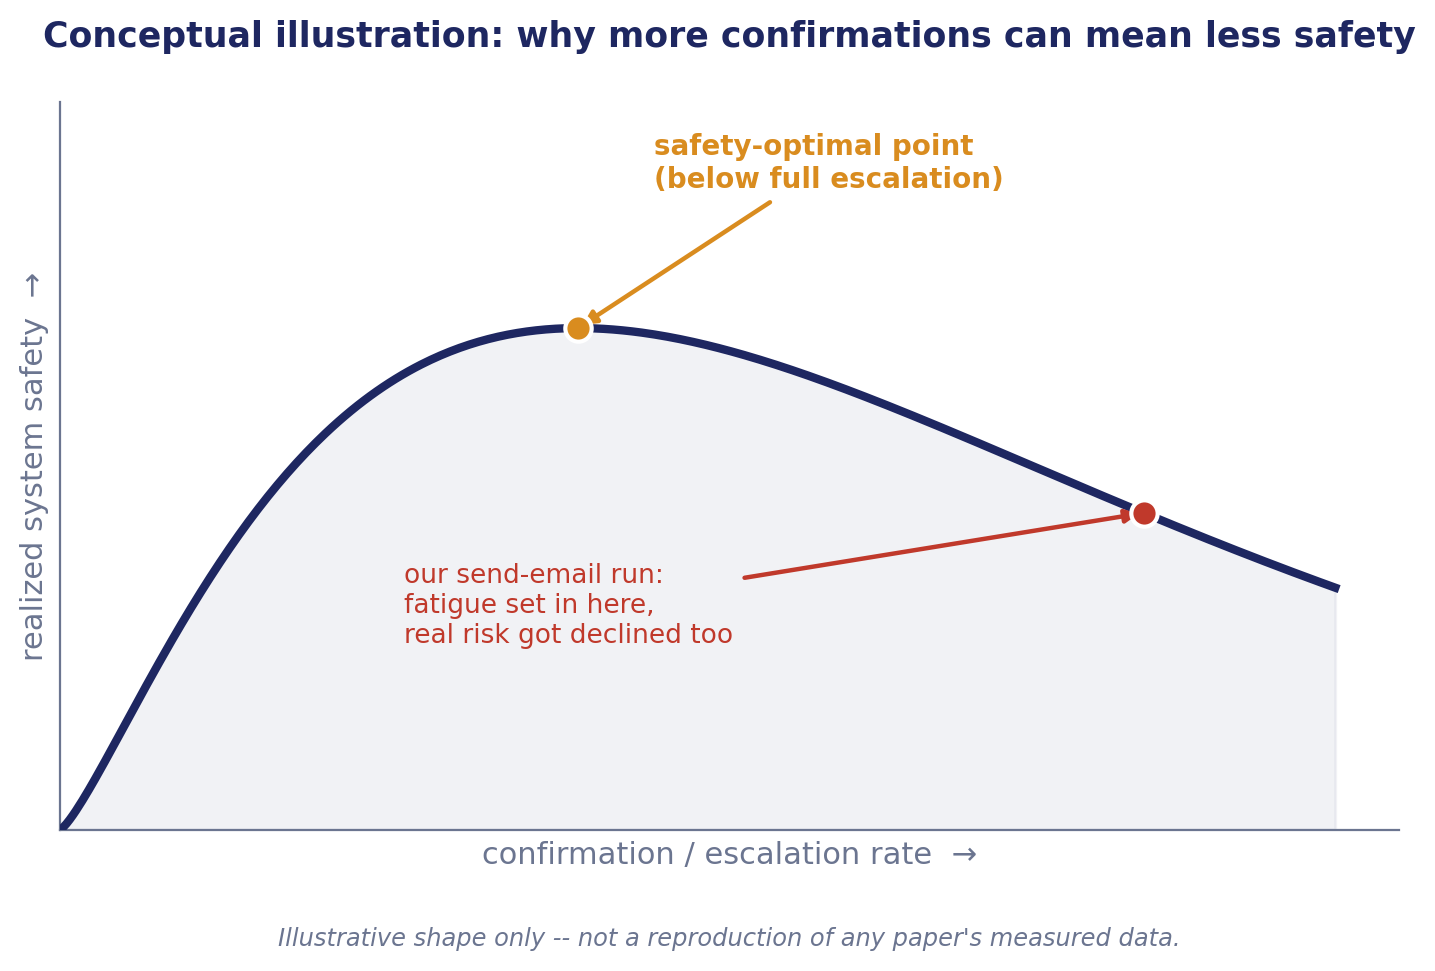
\includegraphics[width=0.75\textwidth]{figures/fig3_inverted_u.png}
  \caption{Conceptual illustration, not a reproduction of Turan (2026)'s measured data, of why realized safety can fall even as the confirmation rate rises: past a point, the human reviewer's attention is the limiting resource, not the check itself. Our send-email run sits roughly where the red marker is -- past the peak.}
  \label{fig:invertedu}
\end{figure}
The closest methodological relative to this work is \textit{Naive Visual Memory is Not Enough}, which proposes AGMem, a general memory mechanism, and evaluates it across three existing GUI-agent benchmarks. Their central finding is a tradeoff: giving the agent full-image memory reduced one category of mistake while making a different category worse. We built nothing comparable in scope -- no new general-purpose mechanism, no multi-benchmark evaluation. What we contribute instead is depth on one real, deployed system: eight failure modes root-caused to a specific mechanism in actual use, not benchmark scores, each verified with a regression test built from the real reasoning text that exposed it. The two studies are not competing on the same axis -- theirs is evidence that a proposed method generalizes across environments, ours is evidence of exactly what broke, and why, in one system that ran for two months. Their tradeoff finding is also directly relevant to our own: the safety-gate asymmetry in \S\ref{sec:mitigation} has the same shape. A single lexical keyword-matching mechanism was, from the start, failing in both directions at once -- missing a genuinely risky Alt+F4 because it never used a listed risk word, and over-firing on unrelated actions that merely mentioned a past failed attempt. Naively tightening that mechanism to catch more real risk would, by construction, also catch more retrospective mentions, worsening the false-positive side exactly as AGMem's full-image memory improved one failure category at the cost of another.
The paper closest to our flagship finding is Turan (2026), \textit{Oversight Has a Capacity}, which formalizes agent safety confirmation as selective classification under asymmetric cost, and shows -- with a measured curve -- that realized safety follows an inverted U as the confirmation rate rises: past a point, the human reviewer's attention becomes the bottleneck, and safety falls even as the system asks for more confirmations. Figure~\ref{fig:invertedu} illustrates this general shape and marks roughly where our own send-email run sits on it, past the peak. We are not claiming priority over this result; it predates our writeup, and Turan's controlled, measured framing is more rigorous than anything we have. What we contribute is a single, real, shipped instance of the same phenomenon, traced to the exact reasoning text that triggered each false confirmation, with a three-layer fix built and measured against that text (\S\ref{sec:mitigation}). A measured curve is the more convincing evidence that this pattern is general; a single grounded run is the more convincing evidence of what it actually looks like when it happens to a live, shipped agent. The two are complementary, not competing.
Three further papers bear on narrower pieces of this taxonomy. OSWorld 2.0 independently reports a stale-coordinate click pattern matching our failure mode 4 (perception-action latency) -- we found this in our own logs before reading their paper, which strengthens rather than undercuts it: two unrelated systems hit the same mechanical failure independently. UI-CUBE, an enterprise benchmark of 226 GUI tasks, reports a sharp capability cliff between simple UI interactions (67--85\% success) and complex multi-step workflows (9--19\% success), attributed to architectural limits in memory, planning, and state coordination rather than prompting quality -- consistent with our own observation that nearly all of our failure modes surfaced in multi-step sequences, not single actions. The LLM-Brained GUI Agents survey is a broad landscape paper mapping frameworks, training data, and evaluation methods across the field; we cite it only to note that the field itself has flagged reliability and evaluation as open problems, not for any specific empirical claim. \textit{What Breaks When LLMs Code?} names a category, ``Safety Guardrail Over-triggering,'' that appears to describe the false-positive direction of our own safety-gate asymmetry under different terminology.
\section{System Description}
\label{sec:system}
Each iteration of the agent's control loop follows five steps, shown in Figure~\ref{fig:loop}. First, the loop captures a screenshot of the current screen and normalizes it before it is used for anything else. Second, the normalized screenshot, the task instruction, and a condensed history of prior steps are sent to a vision-language model -- either Claude or Gemini, depending on configuration -- which returns a single proposed action in a structured format (reasoning, action type, coordinates, and any accompanying text or key). Third, that proposed action passes through a three-layer safety check (\S\ref{sec:mitigation}) before anything happens on the real machine. Fourth, once cleared, the action is carried out on the operating system, primarily through \texttt{pyautogui} for mouse and keyboard control. Fifth, the full record of that iteration -- reasoning, action taken, and outcome -- is appended to the run's log alongside every prior and subsequent iteration, so the next decision step has access to condensed history rather than starting blind.
Architecturally, this loop sits on top of two further layers. The first is the \texttt{VLMBackend} interface: rather than calling one model's API directly from the loop, every model call goes through a common interface, so the same loop logic runs unmodified against Claude, Gemini, or any future backend implementing the same contract -- this is what let us run both backends behind one agent rather than maintaining two separate codepaths. The second is the execution layer, which translates a structured action (click, type, key, scroll, wait, done, fail) into real \texttt{pyautogui} calls against the operating system, and is where deterministic fixes like \texttt{focus\_window} and \texttt{\_bring\_forward\_after\_open()} (\S\ref{sec:results}, mode 8) live.
\begin{figure}[h]
  \centering
  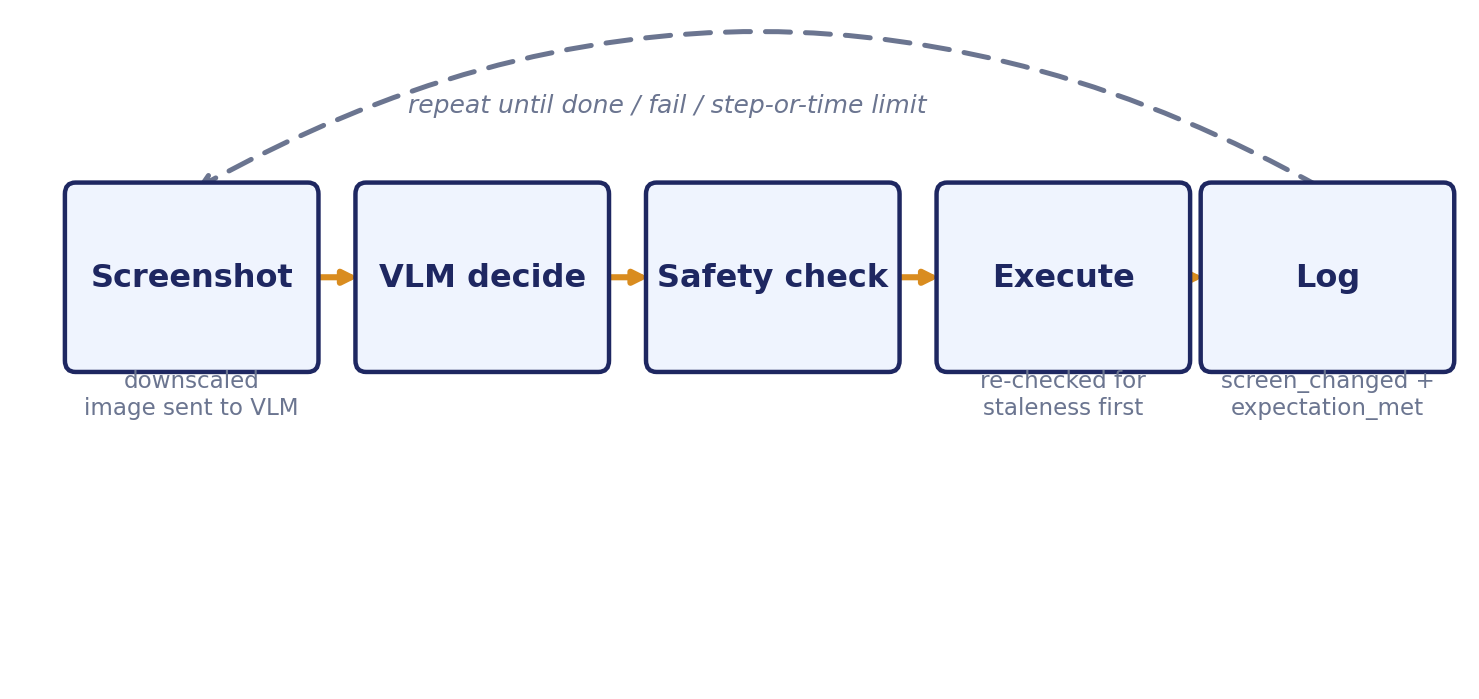
\includegraphics[width=0.95\textwidth]{figures/fig1_loop.png}
  \caption{The five-step control loop, generated from the real loop structure in \texttt{core/loop.py}.}
  \label{fig:loop}
\end{figure}
\section{Methodology}
Each run produced its own timestamped folder containing a per-step log (reasoning, action, coordinates, outcome), full-resolution screenshots, and a summary record, as described in \S\ref{sec:system}. A candidate bug only became one of the eight failure modes once two conditions were met: it recurred rather than being a single unexplained event, and its cause could be pointed to as a specific, persistent flaw in the code or system design -- something that would happen again under the same conditions -- rather than something resolvable by simply re-reading and lightly adjusting code that was already there. That second condition is what separates a failure mode from an ordinary glitch: a glitch is closed by re-examining existing code, a failure mode required the code to actually gain something it was missing -- a check, a translation step, a deterministic action -- not just a tweak.
Verifying a fix meant more than confirming the original failure no longer reproduced -- each fix was also checked against the possibility that it had introduced a new problem elsewhere. Two examples illustrate this. Resizing the screenshot sent to Gemini fixed one problem but, on closer testing, measurably reduced the precision of the model's coordinate guesses -- a tradeoff that would have gone unnoticed without deliberately re-testing accuracy after the change, not just re-testing the original bug. The safety-gate mitigation itself was built through repeated rounds of the same discipline: adding a keyword-based flag list closed the original gap, but retesting surfaced a new problem -- past-tense mentions of an old attempt re-triggering the same flag -- which led to the retrospective-mention filter (Layer 2, \S\ref{sec:mitigation}); retesting that fix in turn surfaced a further gap -- the filter has no real understanding of sentence meaning, only word position -- which is why the self-reported \texttt{risk\_level} field (Layer 3) exists as an independent backstop rather than a fourth layer of keyword tuning.
\section{A Taxonomy of Eight Failure Modes}
\label{sec:results}
\begin{longtable}{|c|P{2.5cm}|P{6.0cm}|P{4.3cm}|}
\hline
\rowcolor{navy}
\textcolor{white}{\textbf{\#}} & \textcolor{white}{\textbf{Failure mode}} & \textcolor{white}{\textbf{Description}} & \textcolor{white}{\textbf{Fix (verified)}} \\
\hline
\endfirsthead
\hline
\rowcolor{navy}
\textcolor{white}{\textbf{\#}} & \textcolor{white}{\textbf{Failure mode}} & \textcolor{white}{\textbf{Description}} & \textcolor{white}{\textbf{Fix (verified)}} \\
\hline
\endhead
\hline
\endfoot
1 & Grounding & Model never told exact downscaled image size; estimates coordinates from priors. & Both backends now state width $\times$ height every turn. \\
\hline
2 & Missing capability & No action to bring an open window to the foreground. & Deterministic \texttt{focus\_window} action, foreground-change verified not assumed. \\
\hline
3 & Safety-gate asymmetry (\S\ref{sec:mitigation}, \S\ref{sec:case-studies}) & Lexical guardrail on reasoning text misses dangerous actions worded around it, AND over-fires on unrelated actions that merely mention a risk word retrospectively. & Three layers: structural key-combo check; retrospective-mention sentence filter; self-reported \texttt{risk\_level} field. \\
\hline
4 & Perception-action latency & Coordinates computed before decision round-trip completes; page can reflow. & Re-screenshot immediately before click; skip if screen changed since decision. \\
\hline
5 & Execution/schema mismatch & "type" action's coordinates were silently ignored by the executor. & "type" with coordinates now clicks that spot first, then types. \\
\hline
6 & Detection sensitivity & Whole-screen diff misses small real changes on a large monitor. & Added localized diff cropped to the action coordinates. \\
\hline
7 & Memory coordinate-space leak & History reported real screen pixels while model reasons in downscaled image space. & History now reports image-space coordinates; real pixels used only for execution. \\
\hline
8 & Background success invisibility (\S\ref{sec:case-studies}) & \texttt{open\_url}/\texttt{launch\_app} can succeed in a window that never gets OS focus; next screenshot looks like failure. & \texttt{\_bring\_forward\_after\_open()} confirms foreground via \texttt{focus\_window}; reports nothing if unconfirmed. \\
\hline
\caption{Eight failure modes found and closed over two months of real use.}
\label{tab:taxonomy}
\end{longtable}
\section{Mitigation: A Layered Fix for the Safety-Gate Asymmetry}
\label{sec:mitigation}
A lexical safety gate -- one that looks for specific words in the model's own explanation of its action -- is only ever a proxy for the model's actual intent, and any proxy built this way fails in both directions at once. Miss enough real risk words and genuinely dangerous actions slip through unconfirmed; add enough words to close that gap and the check starts firing on anything that merely mentions a risk word in passing, including sentences that are only describing something that already happened. Tightening the keyword list to catch more real risk mechanically catches more of these retrospective mentions too -- the two failure directions share the same lever, so pulling on it to fix one makes the other worse. This is why the fix here is not a bigger keyword list, but three independent layers that each catch what the others structurally cannot.

Layer 1 checks the actual key being pressed against a small, fixed list of dangerous key combinations -- Alt+F4, Ctrl+W, Ctrl+Q, Ctrl+Alt+Delete, Win+L -- and does not read the model's reasoning text at all. This exists because of a real run in which the agent pressed Alt+F4 with zero confirmation: its own explanation was ``I need to close this application to proceed,'' which never touched a listed risk word, so no lexical check could ever have caught it. Layer 1 closes that gap by never depending on wording in the first place -- it doesn't matter how the model describes the action, only what the action mechanically is.

Layer 2 is the smarter version of the original keyword check: before scanning reasoning text for risk words, it first discards any sentence containing a retrospective marker -- ``didn't,'' ``failed,'' ``previous attempt,'' and similar phrasing -- so a keyword mentioned only while explaining a past failure no longer re-triggers the check. This closes the gap exposed by the send-email run (\S\ref{sec:case-studies}), where a single real mention of a failed Send click kept getting re-flagged on every later, unrelated action for the rest of the run, because the model kept referencing it while explaining its retries. This heuristic has a known limitation: it is not real tense parsing, so a sentence that mixes a genuinely current risky action with a past-tense reference in the same clause -- for example, ``since deleting it last time failed, I'll delete it again now'' -- can still slip through undetected.

Layer 3 closes exactly that remaining gap, and generalizes across both failure directions at once, because it doesn't depend on any specific wording at all: the model is instructed to fill in a dedicated \texttt{risk\_level} field on every action, rating it honestly as low, medium, or high, independent of whatever words happen to appear in its reasoning. This also closes a separate gap neither of the other two layers could: a run that described sending an email using only ``compose'' or ``submit,'' never the word ``send,'' would have produced zero confirmation if wording were the only signal available.

Figure~\ref{fig:layers} summarizes how the three layers fit together: each is checked in sequence, independent of the others, and any single match is enough to pause the action.
\begin{figure}[h]
  \centering
  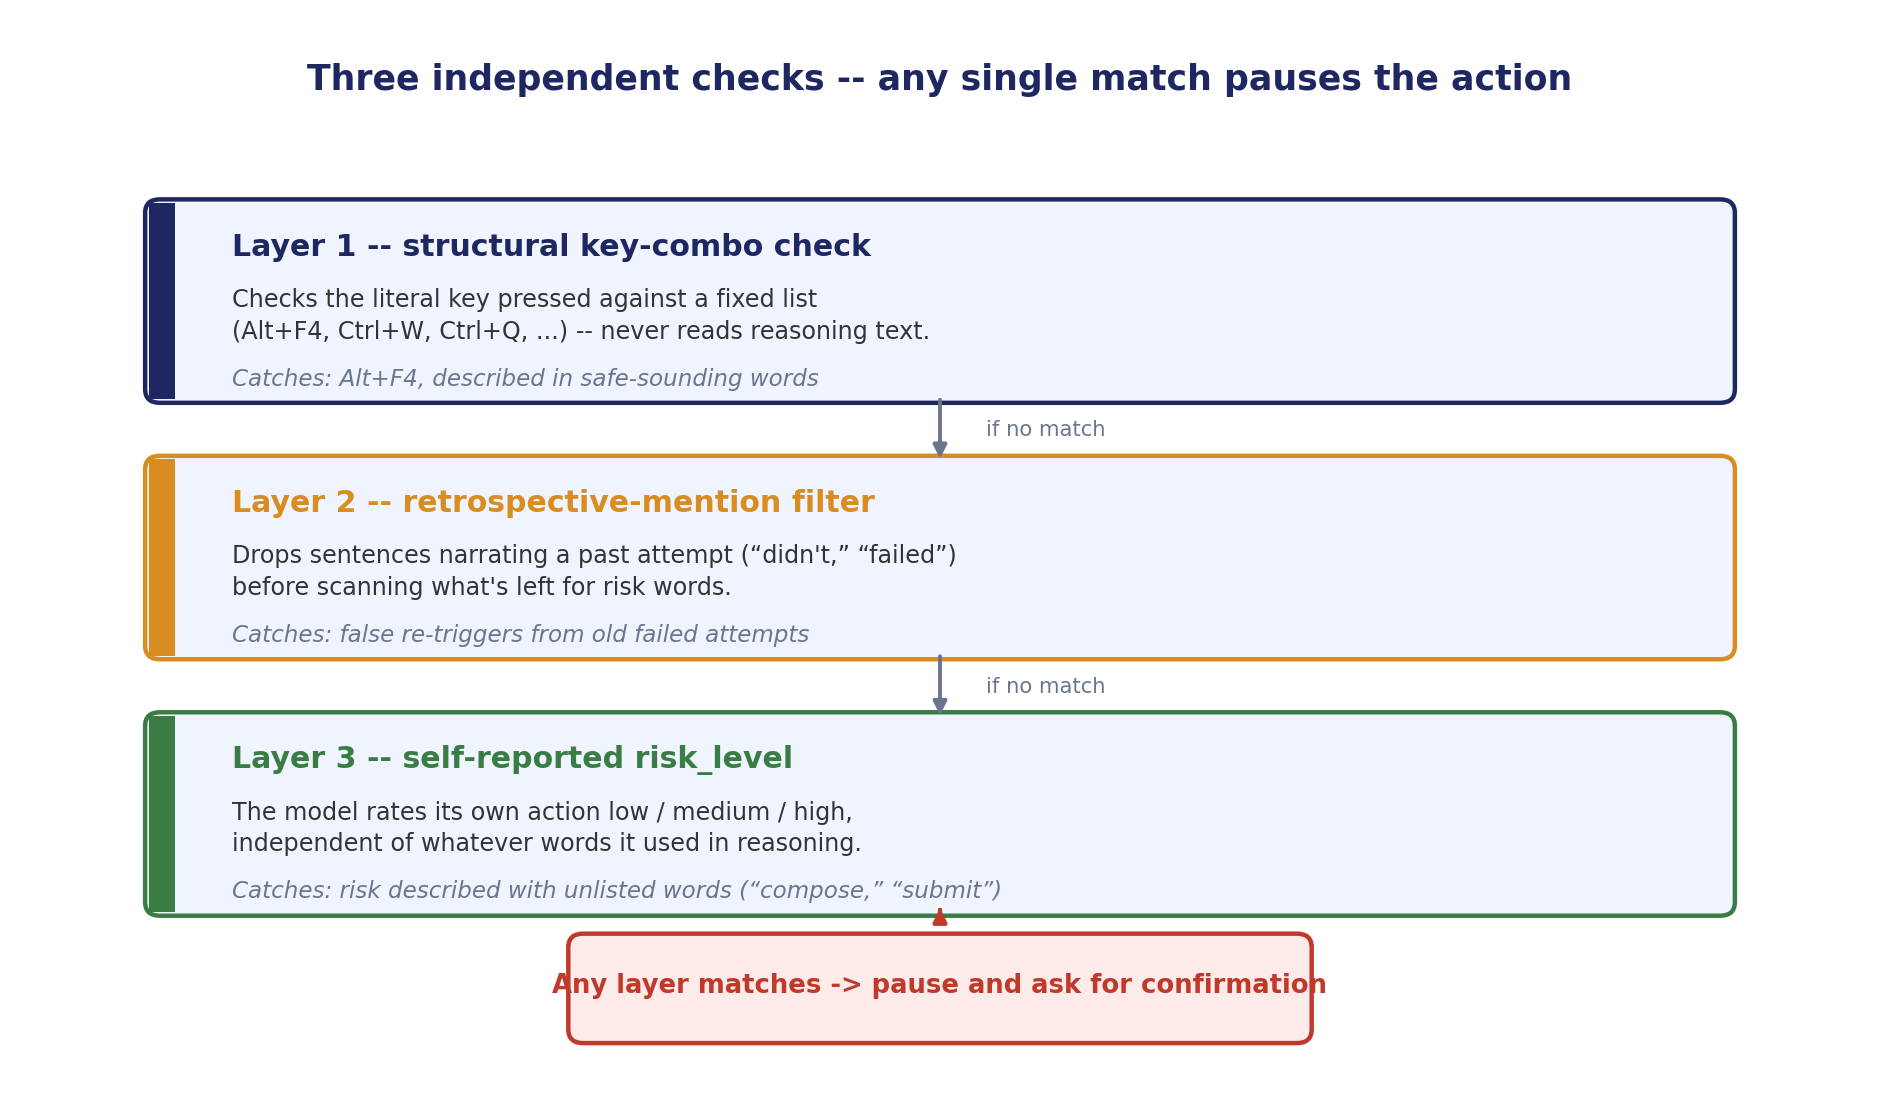
\includegraphics[width=0.85\textwidth]{figures/fig4_layers.png}
  \caption{The three safety-gate layers, checked in sequence -- any single match triggers a confirmation pause.}
  \label{fig:layers}
\end{figure}

Figure~\ref{fig:fatigue} shows the measured effect of Layers 2 and 3 together, built directly from \texttt{tests/test\_retrospective\_filter.py} and run against the exact reasoning text of the send-email run that exposed the bug. Under the original keyword check, steps 10 through 17 of that run -- eight consecutive steps -- all matched a risk word and triggered a confirmation prompt, even though only steps 10 and 14 were genuine attempts to click Send. Under the fixed check, only those two genuine steps still match; the other six, which were only narrating a past failed attempt while retyping the body or closing an unresponsive window, no longer do.
\begin{figure}[h]
  \centering
  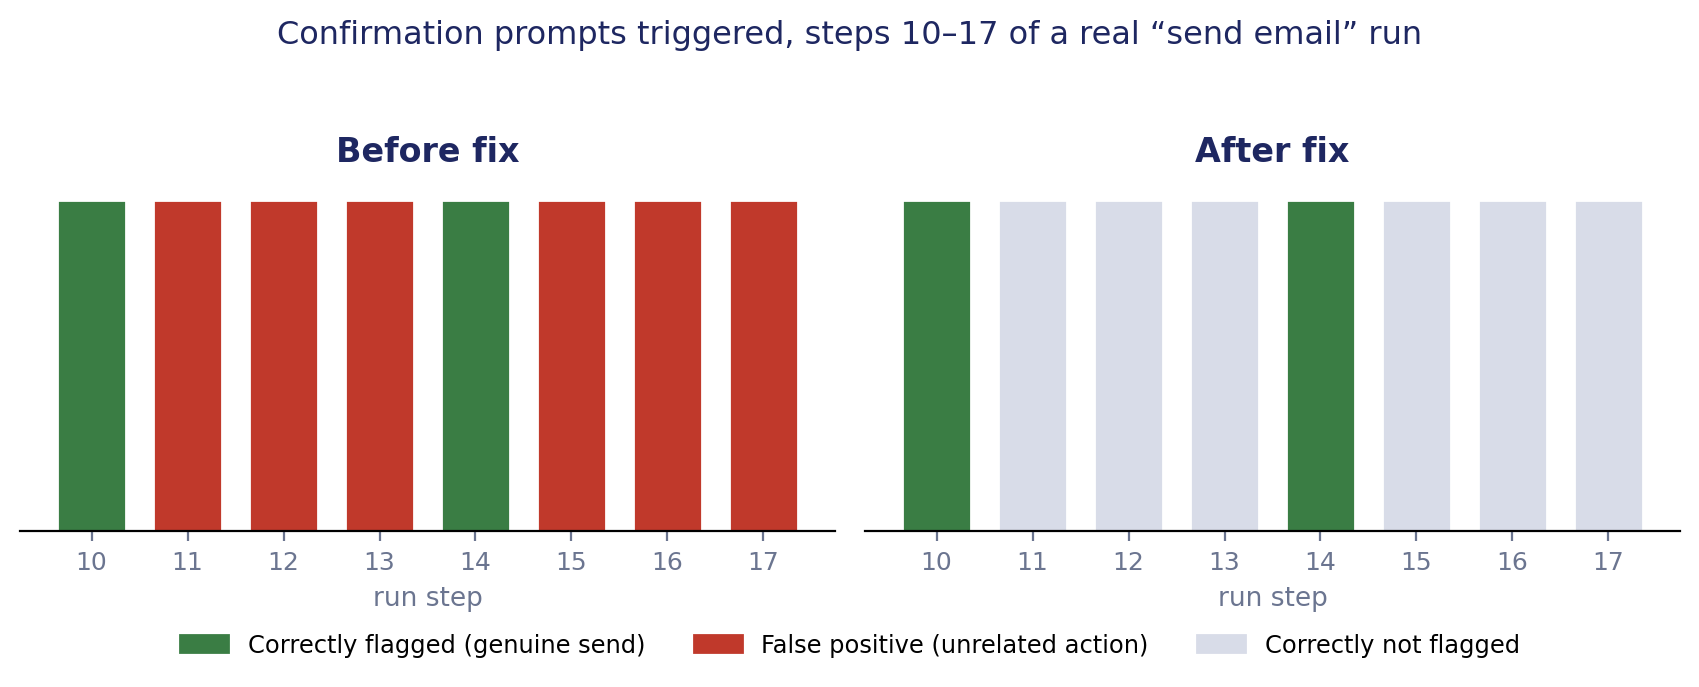
\includegraphics[width=0.92\textwidth]{figures/fig2_fatigue.png}
  \caption{Before/after confirmation counts, steps 10--17 of the real send-email run, measured against the run's exact reasoning text via \texttt{tests/test\_retrospective\_filter.py}.}
  \label{fig:fatigue}
\end{figure}
\section{Case Studies}
\label{sec:case-studies}
\textbf{The Alt+F4 run (false negative).} Asked to switch from a code editor to a browser, the agent decided the fastest path was to close the current application outright. Its full reasoning was functional rather than alarming: it needed to close the application to proceed with opening a browser. Nothing in that sentence matched any word on the safety check's list, so the action executed immediately, with zero confirmation, even though the window in question had unsaved work open. The root cause was structural, not a wording accident: a check built entirely on scanning free-text reasoning for specific words can never catch a dangerous action the model happens to describe in ordinary, functional language. The fix was Layer 1 (\S\ref{sec:mitigation}): a small, fixed list of dangerous key combinations, checked directly against the literal key the agent is about to press, independent of how it explains the action. This closes the gap by construction -- there is no wording left to get around, because none is read.

\textbf{The send-email run (false positive / fatigue cascade).} Composing an email, the agent's first attempt to click Send appeared not to register -- the screenshot showed no change, and the compose window stayed open. From there, the model's reasoning kept referencing that failed attempt while it retried: retyping the body, clicking to refocus the field, eventually closing the unresponsive window and reopening a new compose window. Every one of those seven follow-up steps mentioned the word ``Send'' while explaining what had already gone wrong, and the original keyword check treated every mention the same way, regardless of tense -- triggering a confirmation prompt on each of them. After enough of these, the operator stopped trusting the prompts and declined the one that appeared right before the run was abandoned, without the two genuine send attempts (steps 10 and 14) ever getting a clean, trusted decision. The fix was Layers 2 and 3 together (\S\ref{sec:mitigation}): the retrospective-mention filter stopped past-tense references from re-triggering the check, and the self-reported \texttt{risk\_level} field stands as an independent backstop for whatever the filter's tense heuristic still misses. Figure~\ref{fig:fatigue} shows the measured result: eight flagged steps under the old check, two under the fixed one, matching the two genuine sends exactly.

\textbf{The weather-search run (mode 8).} Asked to look up the weather, the agent used \texttt{open\_url} to open a search directly in the default browser -- and the action genuinely succeeded, opening in a background tab while a separate development environment kept operating-system focus. The next screenshot was accurate, but it showed the dev environment, not the browser, because nothing had actually brought the new tab to the foreground. The model read that screenshot as evidence the action had failed and launched a second, redundant browser window trying to fix something that already worked -- which in turn triggered an unrelated profile-picker dialog neither the model nor the original task ever anticipated. The root cause was a blind spot between what the operating system did and what the agent could perceive: a genuine success is indistinguishable from a failure if the window that succeeded never gets focus. The fix, \texttt{\_bring\_forward\_after\_open()} (\S\ref{sec:system}), waits briefly after \texttt{open\_url} or \texttt{launch\_app} and then confirms the resulting window is actually in the foreground, reporting nothing if it can't be confirmed rather than assuming success. Unlike the other seven fixes in this taxonomy, this one is verified only against mocked tests, not against a second live run on Windows -- a limitation stated plainly in \S\ref{sec:limitations}.
\section{Discussion}
Not all eight failure modes sit at the same level. Four of them -- grounding (mode 1), missing capability (mode 2), execution/schema mismatch (mode 5), and detection sensitivity (mode 6) -- are implementation-level: each was a specific, contained gap in what the code did, closed by adding one missing piece of information or one missing step, without touching how the agent is structured overall. The other four -- safety-gate asymmetry (mode 3), perception-action latency (mode 4), memory coordinate-space leak (mode 7), and background success invisibility (mode 8) -- are architecture-level: each reflects a structural blind spot in how the loop perceives, reasons about, or acts on state, and closing them required the system to gain a genuinely new mechanism (three safety layers, a re-screenshot check, a consistent coordinate space, a foreground-confirmation step) rather than a single contained patch.

OSWorld 2.0's independent report of the same stale-coordinate click pattern behind mode 4 is weak evidence on its own -- one other paper, using a different system, a different benchmark, a different methodology -- but it is real evidence, and two unrelated systems converging on the same mechanical failure without either team reading the other's work is harder to dismiss as a one-off quirk of this particular codebase.

The comparison to Turan (2026) is worth stating plainly rather than glossing over. Turan's evidence is a measured curve, built from controlled trials across many data points, and is the stronger evidence that oversight fatigue is a general phenomenon. What this paper offers is different in kind, not degree: one real, dated, root-caused instance of that exact phenomenon inside a live, shipped system, with a fix built and measured against the precise reasoning text that exposed it. Neither kind of evidence replaces the other -- a controlled study proves a pattern is real and general; a grounded case proves what that pattern actually looks like, mechanically, when it happens to a system someone actually built and ran.
\section{Limitations}
\label{sec:limitations}
\begin{datanote}
Of the 15 runs with \texttt{status: "fail"} in the corpus, 14 were caused by external dependencies -- Gemini API rate limits (429 RESOURCE\_EXHAUSTED), daily free-tier quota exhaustion across all configured API keys, a DNS resolution failure (\texttt{getaddrinfo failed}), a 503 from the model provider, and one dropped SSL connection. Only 1 of the 15 \texttt{fail}-status runs reflects a genuine agent-level failure (a Gmail compose-window run that exhausted its retries). None of this is a failure of the agent's own reasoning or of the harness code around it -- it's the deployment environment underneath both.
\end{datanote}
This taxonomy is qualitative, not statistically validated: it comes from reading 91 logged runs in full, not from a benchmark scored automatically at scale. Two of the eight modes -- the fatigue direction of the safety-gate asymmetry (mode 3) and background success invisibility (mode 8) -- rest on a smaller evidence base than the other six, drawn from a later, separate batch of runs rather than the core corpus, and mode 8's fix is verified only against mocked tests, not a second live run on Windows. The task distribution is narrow, concentrated mostly on browser and Gmail workflows; the system has only been run on one operating system, behind two model backends, and every run was read and classified by a single annotator with no independent second reviewer. The safety-gate asymmetry finding, while discovered independently through this project's own runs, is not the first documented instance of agent-oversight fatigue -- Turan (2026) treats the same underlying pattern formally and predates this writeup (\S\ref{sec:related}).

Most non-``done'' runs in this corpus did not fail because of anything this taxonomy covers. Of the 15 runs with a fail status, 14 were caused by external dependencies -- API rate limits, quota exhaustion, a DNS failure, a provider outage, a dropped connection -- not by any flaw in the agent's reasoning or the code around it. Only one reflects a genuine agent-level failure. That distinction matters: the raw per-run status numbers alone would make it look like the agent failed far more often than it actually did on its own account, when in fact the large majority of incomplete runs reflect the deployment environment underneath it, a different category of problem entirely from anything in this paper's eight modes.
\section{Future Work}
\label{sec:future}
A 16-task benchmark harness already exists in this codebase but has not yet been run end-to-end; a subset of it was built specifically to stress mode 8 more rigorously than the single weather-search run this paper reports, and running it is the most direct way to move that mode off its current, thinner evidence base. A deeper fix for mode 1 is also worth pursuing: rather than only telling the model the exact size of the image it's shown, grounding could be improved further with OCR or accessibility-tree information, giving the model actual element boundaries to reason over instead of only pixel estimates.

Two open questions follow directly from this paper's central finding rather than from it. First, whether the safety-gate asymmetry recurs across models with different reasoning styles is untested here -- this system ran behind two backends, but both were checked with the same lexical mechanism, so it remains an open question rather than a claim whether a model with a different way of narrating its own reasoning would expose the same gap in the same way. Second, Turan (2026)'s formal inverted-U framing was never applied directly to this system's own run data -- doing so, rather than relying on a single dated run and a conceptual illustration (Figure~\ref{fig:invertedu}), would be a natural follow-up measurement connecting this paper's grounded case to Turan's more general model.
\section{Conclusion}
A safety mechanism's failure rate has to be measured in both directions at once, because a fix that only reduces missed risks can just as easily make false alarms -- and the fatigue they cause -- worse in the same breath. This paper documented that exact pattern end to end in one real, shipped system: a lexical safety gate that let a genuine risk through unconfirmed in one run, and flooded an unrelated, harmless sequence with confirmations in another, through the same underlying mechanism. The three-layer fix built here closed both directions at once, verified against the precise reasoning text of the run that exposed the problem, not against a synthetic benchmark. This is one grounded, shipped instance of a pattern the field is actively formalizing elsewhere (Turan, 2026), not a claim to have discovered it first. What a reader should take away is not confidence in this exact codebase, but the underlying discipline: check a safety fix in both directions, on real data, before trusting that it made anything safer.
\section*{References}
\addcontentsline{toc}{section}{References}
\begin{enumerate}[leftmargin=1.6em, itemsep=0.3em]
  \item Naive Visual Memory is Not Enough: A Failure-Mode Study of GUI Agents. arXiv:2606.14106. \url{https://arxiv.org/pdf/2606.14106}
  \item Turan, E. (2026). Oversight Has a Capacity: Calibrating Agent Guards to a Subjective, Fatiguing Human. arXiv:2606.08919. \url{https://arxiv.org/abs/2606.08919}
  \item OSWorld 2.0: Benchmarking Computer Use Agents on Long-Horizon Real-World Tasks. arXiv:2606.29537. \url{https://arxiv.org/html/2606.29537v1}
  \item UI-CUBE: Enterprise-Grade Computer Use Agent Benchmarking Beyond Task Accuracy to Operational Reliability. arXiv:2511.17131. \url{https://arxiv.org/pdf/2511.17131}
  \item Large Language Model-Brained GUI Agents: A Survey. arXiv:2411.18279. \url{https://arxiv.org/pdf/2411.18279}
  \item What Breaks When LLMs Code? Characterizing Operational Safety Failures of Agentic Code Assistants. arXiv:2605.30777. \url{https://arxiv.org/pdf/2605.30777}
  \item Akhawe, D., \& Felt, A. P. (2013). Alice in Warningland: A Large-Scale Field Study of Browser Security Warning Effectiveness. \textit{Proceedings of the 22nd USENIX Security Symposium}, 257--272.
\end{enumerate}
\vspace{0.5em}
\noindent\textit{Primary sources (project data):}
\begin{enumerate}[leftmargin=1.6em, itemsep=0.3em]
  \item Vision-Language Desktop Agent -- source code and README.
  \item \texttt{runs/} directory -- raw logged run data underlying Sections~\ref{sec:results}--\ref{sec:case-studies}.
  \item \texttt{tests/} directory -- 81 regression tests, including \texttt{test\_retrospective\_filter.py}, built from the real reasoning text behind \S\ref{sec:mitigation}.
\end{enumerate}
\end{document}
